\documentclass{elsarticle}
\usepackage{graphicx}
%\usepackage{multicol}
%\usepackage{footmisc}
\usepackage{amstext}
\usepackage{amsmath}
\usepackage{amssymb}
\usepackage[english]{babel}
%\usepackage[official,right]{eurosym}
\selectlanguage{english}
% Ampersand -----------------------------------------------------------

\def\id#1{\text{\em #1\/}}
\newcommand{\code}[1]{\text{\tt\small #1}}
\newcommand{\stmtText}[1]{``{\small\tt #1}''}
\newcommand{\dom}[1]{\id{dom}(#1)}
\newcommand{\cod}[1]{\id{cod}(#1)}
\renewcommand{\int}[2]{\id{inter}(#1,#2)}
\newcommand{\pop}[1]{\id{pop}(#1)}
\newcommand{\src}[1]{\id{src}(#1)}
\newcommand{\trg}[1]{\id{trg}(#1)}
\newcommand{\powerset}[1]{\cal{P}\{#1\}}
\newcommand{\theCode}{\url{http://cs.ru.nl/~B.Joosten/ampTypes/}}
\newcommand{\la}{\langle}
\newcommand{\ra}{\rangle}
\newcommand{\full}{V}
\newcommand{\declare}[3]{\id{#1}_{\pair{\id{\small #2}}{\id{\small #3}}}}
\newcommand{\fullt}[2]{V_{\pair{#1}{#2}}}
\newcommand{\iden}[1]{I}
\newcommand{\ident}[1]{I_{\id{\small #1}}}
\newcommand{\expr}[3]{(#1)_{#2\times #3}}
\newcommand{\pair}[2]{\la{#1},{#2}\ra}
\newcommand{\atom}[1]{{\tt\small #1}}
\newcommand{\atoms}{\mathcal{A}}
\newcommand{\concepts}{\mathcal{C}}
\newcommand{\decls}{\mathcal{D}}  %% names of relations
\newcommand{\rels}{\mathcal{R}}   %% all relations
\newcommand{\relations}{\mathcal{M}} % representing terms. M is a subset of R.
\newcommand{\terms}{\mathcal{T}}
\newcommand{\vertices}{N}
\newcommand{\rules}{\mathcal{H}}
\newcommand{\tf}[1]{\mathfrak{T}(#1)}
\newcommand{\ptf}[1]{\mathfrak{T}'(#1)}
\newcommand{\ti}[1]{\mathfrak{I}(#1)}
\newcommand{\tic}[1]{I_{\cal C}(#1)}
\newcommand{\relAdd}{\dagger}
\newcommand{\flip}[1]{{#1}^\smallsmile} %formerly:  {#1}^\backsim
\newcommand{\kleeneplus}[1]{{#1}^+}
\newcommand{\kleenestar}[1]{{#1}^*}
\newcommand{\cmpl}[1]{\overline{#1}}
\newcommand{\rel}{\times}
\newcommand{\compose}{;}
\newcommand{\subs}{\subseteq}%{\models}
\newcommand{\fun}{\rightarrow}
\newcommand{\isa}{\preceq}
%\newcommand{\isaClos}{\sqsubseteq}
\newcommand{\typetest}{?}
\newcommand{\meet}{\sqcap}
\newcommand{\join}{\sqcup}
\newcommand{\Meet}{\bigsqcap}
\newcommand{\Moin}{\bigsqcup} % because LaTeX has already defined command \Join.
\newcommand{\order}{\ominus}
\newcommand{\anything}{\top}
\newcommand{\nothing}{\bot}
\newcommand{\rewriteto}{\rightarrow}
\newcommand{\calc}{\implies}
\newcommand{\alland}{\bigwedge}
\newcommand{\mph}[3]{#1_{#2\times #3}}
\newcommand{\mphu}[1]{#1_{\univ\times\univ}}

%-----------------------------------------
\newcommand{\kse}{\hspace*{1.7em}}
\newcommand{\ksf}{\hspace*{1em}}
\newcommand{\ksg}{\hspace*{1em}}
\newenvironment{derivation}{\begin{tabbing}\kse \= \ksf \= \ksg \= \kill}{\end{tabbing}}
\newtheorem{definition}{Definition}
\newcommand{\term}[1]{\>\>\(#1\)\\[1ex]}
\newcommand{\rela}[2]{\>\(#1\)\>\>\{ \ #2 \ \}\\[1ex]}
\newcommand{\weg}[1]{}

\def\define#1{\label{dfn:#1}{\em #1}\index{#1}}
\def\definem#1{\label{dfn:#1}{\em #1}\index{#1}\marge{#1}}
\newcommand{\marg}[1]{\index{#1}\marge{#1}}

\hyphenation{ExecEngine}
\begin{document}

\title{A Theory for Database Transactions with no Database}
\author[ou,ordina]{Stef Joosten\fnref{fn1}}
\ead{stef.joosten@ou.nl}
\address[ou]{Open Universiteit Nederland, Postbus 2960, 6401 DL Heerlen, the Netherlands}
\address[ordina]{Ordina NV,  Nieuwegein, the Netherlands}
\fntext[fn1]{ORCID 0000-0001-8308-0189}

\begin{abstract}
	How to do transactions if data is scattered across the internet?
	Users who must satisfy data integrity constraints are stuck with relational databases if they need transactions.
	For most NoSQL databases lack transaction functionality.
	This contribution proposes a theory of database transactions solely based on data,
	with no reference to any database in which that data resides.
	This makes transactions suitable for a wider class of databases than just relational ones.
	The soundness of the theory has been established by means of category theory.
	To show that the theory works, the theory is demonstrated by a prototype developed in Ampersand\footnote{\tt https://github.com/AmpersandTarski/Ampersand}.
	To demonstrate that the theory is about real transactions, this contribution defines semantics of conventional database transactions.
	To fulfill our promise, we also gives semantics of transactions on the semantic web.
\end{abstract}

\begin{keyword}
relation algebra\sep software development\sep legal reasoning\sep information systems design\sep Ampersand\sep MirrorMe\sep reactive programming
\end{keyword}
\maketitle

\section{Introduction}
\label{sct:Introduction}

\section{Consistency}
\label{sct:Consistency}
	Each user of a database issues a stream of events.
	The order (in time) of events is given by a relation\footnote{%
A relation $\declare{r}{A}{B}$ is a set of tuples $\pair{a}{b}$ with $a\in A$ and $b\in B$} $\declare{pred}{Event}{Event}$,
	where $\pair{e1}{e2}\in\id{pred}$ means that event $e1$ precedes event $e2$.
	From a user perspective this stream is a sequence, so every event except the first has exactly one predecessor.
	
	For simplicity's sake, we assume the user sees a finite set of items at any given moment.
	The items seen by the user at any moment are given by a relation $\declare{state}{Event}{Item}$,
	where $\pair{e}{i}\in\id{state}$ means that item $i$ exists immediately after $e$ has occured.
	So the set of items visible to the user immediately after $e$ has occured can be computed by $\{ i | \pair{e}{i}\in\id{state} \}$.
	Note that the relation $\id{state}$ is interpreted in an open world.
	If $\pair{e}{i}\not\in\id{state}$ this does not mean $i$ does not exist.
	It just means that the pair $\pair{e}{i}$ is not in $\id{state}$, so the user will not see it.

	To cope with change, a user may insert and/or delete items at will.
	Let us specify these deletions and insertions by two relations, $\declare{ins}{Event}{Item}$ and $\declare{del}{Event}{Item}$,
	where $\pair{e}{i}\in\id{ins}$ means that pair $\pair{e}{i}$ is to be added to $\id{state}$,
	and $\pair{e}{i}\in\id{del}$ means that pair $\pair{e}{i}$ is to be removed from $\id{state}$.
	More precisely, let us consider an event $e$.
	The items $\{ i | \pair{e}{i}\in\id{state} \}$ are the items that exist immediately after the preceding event has occured,
	minus the items to be removed, plus the items to be inserted.
	The following equation defines this \define{behaviour}:
\begin{equation}
	\id{state}\ =\ (\id{pred};\id{state}-\id{del})\cup\id{ins}
\label{behaviour}
\end{equation}
	Equation~\ref{behaviour} says that the items visible to the user immediately after an event $e$
	are all items that are inserted together with items that were visible immediately after the preceding event, except those that were deleted.

	We define $A_{(\id{ins},\id{del})}$ as the function\footnote{The name $A$ is chosen as a reminder to the word ``action''.}
	that embodies this change:
\begin{equation}
	A_{(\id{ins},\id{del})}(x)\ =\ (x-\id{del})\cup\id{ins}
\end{equation}

	This raises the question whether we can compose two actions into a single action.
	For this, we derive:
\[\begin{array}{r@{~}l}
	&(((x-\id{del})\cup\id{ins})-\id{del}')\cup\id{ins}'\\
	=&\hspace{1in}\{x-y=x\cap\overline{y}\}\\
	&(((x\cap\overline{\id{del}})\cup\id{ins})\cap\overline{\id{del}'})\cup\id{ins}'\\
	=&\hspace{1in}\{\text{distribute $\cap$ over $\cup$}\}\\
	&(x\cap\overline{\id{del}}\cap\overline{\id{del}'})\cup(\id{ins}\cap\overline{\id{del}'})\cup\id{ins}'\\
	=&\hspace{1in}\{\text{De Morgan}\}\\
	&(x-(\id{del}\cup\id{del}'))\cup(\id{ins}-\id{del}')\cup\id{ins}'\\
	=&\hspace{1in}\{\text{Assume}\ \id{ins}\cap\id{del}=\emptyset\ \text{and}\ \id{ins}'\cap\id{del}'=\emptyset\}\\
	&(x-(\id{del}\cup\id{del}'))\cup(\id{ins}\cup\id{ins}')
\end{array}\]
	This yields composition ($;$) of $A$:
\begin{equation}
	A_{(\id{ins},\id{del})}\ ;\ A_{(\id{ins}',\id{del}')}\ =\ A_{((\id{ins}-\id{del}')\cup\id{ins}', \id{del}\cup\id{del}')}
\label{composition of A}
\end{equation}
	
	The composition operator turns out to be commutative, but under a condition.
	This will appear to be useful later on in this paper.
	Equation~\ref{composition of A} shows that we only need to investigate commutativity in the first argument of $A$: 
\[\begin{array}{r@{~}rcl}
	&A_{(\id{ins},\id{del})}\ ;\ A_{(\id{ins}',\id{del}')}&=&A_{(\id{ins}',\id{del}')}\ ;\ A_{(\id{ins},\id{del})}\\
	\Leftrightarrow\\
	&A_{((\id{ins}-\id{del}')\cup\id{ins}', \id{del}\cup\id{del}')}&=&A_{((\id{ins}'-\id{del})\cup\id{ins}, \id{del}'\cup\id{del})}\\
	\Leftrightarrow\\
	&(\id{ins}-\id{del}')\cup\id{ins}'&=&(\id{ins}'-\id{del})\cup\id{ins}\\
	\Leftrightarrow\\
	&(\id{ins}\cap\overline{\id{del}'})\cup\id{ins}'&=&(\id{ins}'\cap\overline{\id{del}})\cup\id{ins}\\
	\Leftrightarrow\\
	&(\id{ins}\cup\id{ins}')\cap(\overline{\id{del}'}\cup\id{ins}')&=&(\id{ins}\cup\id{ins}')\cap(\overline{\id{del}}\cup\id{ins})\\
	\Leftrightarrow\\
	&(\id{ins}\cup\id{ins}')-\overline{\overline{\id{del}'}\cup\id{ins}'}&=&(\id{ins}\cup\id{ins}')-\overline{\overline{\id{del}}\cup\id{ins}}\\
	\Leftrightarrow\\
	&\id{del}'\cap\overline{\id{ins}'}&=&\id{del}\cap\overline{\id{ins}}\\
	\Leftrightarrow\\
	&\id{del}'-\id{ins}'&=&\id{del}-\id{ins}
\end{array}\]
	For the purpose of making commutativity independent of its arguments,
	we must check the condition $\id{del}'-\id{ins}'=\id{del}-\id{ins}$.

\section{Isolation}
\label{sct:Isolation}
	If a user were alone,
	The moment a transaction starts, its user is isolated from other users.
	That moment is represented by a relation $\declare{beginTransaction}{Event}{Transaction}$,
	where $\pair{e}{t}\in\id{beginTransaction}$ means that event $e$ marks the start of transaction $t$.


\section{Ampersand}
\label{sct:Ampersand}
	In this section we explain the basics of Ampersand.
	The reader is expected to have sufficient background in relation algebra to understand the remainder of this paper.

	The core of an Ampersand script is a triple $\la\rules,\rels,\concepts\ra$,
	which consists of a set of rules $\rules$, relations $\rels$, and concepts $\concepts$.
	An Ampersand script is interpreted by the compiler as an information system.
	The rules constitute a theory in heterogeneous relation algebra.
	They constrain a body of data that resides in a database.

	The Ampersand compiler generates a database from relations in the script.
	A database application%
\footnote{Ampersand generates an application that consists of a relational database and interface components.
	Currently this application runs server-side on a PHP/MySQL platform and on a web-browser on the client-side.}
	assists users to keep rules satisfied throughout the lifetime of the database. It is also generated by Ampersand.

	A rule is a constraint in the form of an equality between two terms.
	Terms are built from relations.
	Ampersand interprets every relation as a finite set of pairs, which are stored in the database.
	The phase in which Ampersand takes a script and turns it into a database, is what we will refer to as \define{compile-time}.
	The phase in which a user interacts with the database, is what we will refer to as \define{run-time}.
	At run-time, Ampersand can decide which rules are satisfied by querying the database.
	The compiler generates all software needed to keep rules satisfied at run-time.
	If one of the rules is not satisfied as a result of data that has changed,
	that change is reverted (rolled back) to the original state.
	Either way, Ampersand ensures that all rules remain satisfied.
	
	Atoms are values that have no internal structure, meant to represent data elements in a database.
	From a business perspective, atoms are used to represent concrete items of the world,
	such as \atom{Peter}, \atom{1}, or \atom{the king of France}.
	By convention throughout the remainder of this paper, variables $a$, $b$, and $c$ are used to represent \emph{atoms}.
	The set of all atoms is called $\atoms$.
        Each atom is an instance of a \emph{concept}.

	Concepts (from set $\concepts$) are names we use to classify atoms in a meaningful way.
	For example, you might choose to classify \atom{Peter} as a person, and \atom{074238991} as a telephone number.
        We will use variables $A$, $B$, $C$, $D$ to represent concepts.
	The term $\ident{A}$ represents the \emph{identity relation} of concept $A$.
	The expression $a \in A$ means that atom $a$ is an \emph{instance} of concept $A$.
	The declaration of $A\isa B$ (pronounce: $A$ is a $B$)
	in an Ampersand script states that any instance of $A$ is an instance of $B$ as well.
	We call this {\em specialization}, but it is also known as {\em generalization} or {\em subtyping}.
	Specialization is needed to allow statements such as: ``An orange is a fruit that ....''.
	Specialization is not used in the remainder of this paper.

	Relations (from set $\rels$) are used in information systems to store data.
%	A \define{fact} is a statement that is true in a business context.
%	Facts are stored and kept as data in a computer.
	As data changes over time, so do the contents of these relations.
	In this paper relations are represented by variables $r$, $s$, and $d$.
	We represent the declaration of a relation $r$ by $\declare{nm}{A}{B}$,
	in which \id{nm} is a name and $A$ and $B$ are concepts.
	We call $A$ the source concept and $B$ the target concept of the relation.
	The pair $\pair{A}{B}$ is called the \emph{type} of the relation.
	The term $\fullt{A}{B}$ represents the \emph{universal relation} over concepts $A$ and $B$.

	The meaning of relations in Ampersand is defined by an interpretation function $\mathfrak{I}$.
	It maps each relation to a set of pairs.
	The type system of Ampersand guarantees that each pair in $r$ respects the type of $r$:
\begin{equation}
	\pair{a}{b}\in\ti{\declare{nm}{A}{B}} \Rightarrow\ a \in A \wedge b \in B \label{typing of relations}
\end{equation}
	The type system is strong, which means that every atom has a type.
	The type system is static, which means that type checking is entirely done at compile-time.

	Terms are used to combine relations using operators.
	The set of terms is called $\terms$.
\begin{definition}[terms]
\label{def:terms}
\item   The set of terms, $\terms$, is the smallest set that satisfies, for all $r,s \in \terms$, $d\in\rels$ and $A,B \in \concepts$: 
\begin{eqnarray}
	d&\in&\terms         \quad\quad\text{(every relation is a term)}\\
	(r \cup s)&\in&\terms\quad\quad\text{(union)}\\
	(r \cap s)&\in&\terms\quad\quad\text{(intersection)}\\
	(r-s)&\in&\terms     \quad\quad\text{(difference)}\label{def:difference}\\
	(r;s)&\in&\terms     \quad\quad\text{(composition)}\\
	(r\backslash s)&\in&\terms     \quad\quad\text{(right residual)}\\
	(r\slash s)&\in&\terms     \quad\quad\text{(left residual)}\\
	\flip r&\in&\terms   \quad\quad\text{(converse)}\\
	\cmpl{r}&\in&\terms   \quad\quad\text{(complement)}\\
%	\kleeneplus r&\in&\terms   \quad\quad\text{(Kleene closure)}\\
%	\kleenestar r&\in&\terms   \quad\quad\text{(Kleene closure)}\\
	\ident{A}&\in&\terms \quad\quad\text{(identity)}\\
	\fullt{A}{B}&\in&\terms \quad\quad\text{(full set)}
\end{eqnarray}
\end{definition}
	Throughout the remainder of this paper,	terms are represented by variables $r$, $s$, $d$, and $t$.
	The \define{type} of a term $r$ is a pair of concepts, given by $\tf{r}$.
	$\mathfrak{T}$ is a partial function that maps terms to types.
	If a term has one type, it is called \define{type correct}.
	The Ampersand compiler requires all terms to be type correct.
	If no type can be assigned, the compiler gives an error message.
	If multiple types are assignable to a term, the ambiguity is signalled by the compiler.
	In that case it will also emit an error message and prompt the programmer to disambiguate the term by adding type information.
	In practice, the derivation of types can disambiguate most terms.
	So, the programmer experiences some freedom to denote distinct relations by the same name without the obligation to specify their types at all occurrences.
	The compiler does not generate any code if there is a term that is not type correct.
	The type function and its restrictions are discussed in~\cite{Joosten2015}
	and have no consequences for the remainder of this paper.

 	The meaning of terms in Ampersand is given by an interpretation function $\mathfrak{I}$.
	Let $A$ and $B$ be finite sets of atoms, then $\mathfrak{I}$ maps each term to the set of pairs for which that term stands.
\begin{definition}[interpretation of terms]
\label{interpretation of terms}
\item   For every $A,B\in\concepts$ and $r,s\in\terms$
\begin{eqnarray}
	\ti{r}		 &=&\{\pair{a}{b}|\ a\ r\ b\}	\\
	\ti{r \cup s}	 &=&\{\pair{a}{b}|\ \pair{a}{b}\in\ti{r}\ \text{or }\ \pair{a}{b}\in\ti{s}\}	\\
	\ti{r \cap s}	 &=&\{\pair{a}{b}|\ \pair{a}{b}\in\ti{r}\ \text{and}\ \pair{a}{b}\in\ti{s}\}	\\
	\ti{r-s}	 &=&\{\pair{a}{b}|\ \pair{a}{b}\in\ti{r}\ \text{and}\ \pair{a}{b}\notin\ti{s}\}	\\
	\ti{r;s}	 &=&\{\pair{a}{c}|\ \text{for some}\ b,\ \pair{a}{b}\in\ti{r}\ \text{and}\ \pair{b}{c}\in\ti{s}\}	\\
	\ti{r\backslash s}	 &=&\{\pair{b}{c}|\ \text{for all}\ a,\ \pair{a}{b}\in\ti{r}\ \text{implies}\ \pair{a}{c}\in\ti{s}\}	\\
	\ti{r\slash s}	 &=&\{\pair{a}{b}|\ \text{for all}\ c,\ \pair{b}{c}\in\ti{s}\ \text{implies}\ \pair{a}{c}\in\ti{r}\}	\\
	\ti{\flip{r}}	 &=&\{\pair{b}{a}|\ \pair{a}{b}\in\ti{r}    \}	\\
	\ti{\cmpl{\declare{r}{A}{B}}}	 &=&\fullt{A}{B}-r	\\
%	\ti{\kleeneplus{r}}	 &=&\text{the smallest set that satisfies }\kleeneplus{r}=r\ \cup\ \kleeneplus{r};\kleeneplus{r}	\\
%	\ti{\kleenestar{\declare{r}{A}{A}}}	 &=&\ident{A}\cup\kleeneplus{r}\\
	\ti{\ident{A}} 	 &=&\{\pair{a}{a}|\ a\in A\}	\\
	\ti{\fullt{A}{B}}&=&\{\pair{a}{b}|\ a\in A, b\in B\}
\end{eqnarray}
\end{definition}
%	The Kleene closure operators (postfix $\kleeneplus{\ }$ and $\kleenestar{\ }$) have been implemented partially in the current Ampersand implementation.

	A \define{rule} is a pair of terms $r,s\in\terms$ with $\tf{r}=\tf{s}$, which is syntactically recognizable as a rule.
\[\text{RULE}\ r = s\]
	This means \(\ti{r} = \ti{s}\). In practice, many rules are written as:
\[\text{RULE}\ r\subs s\]
	This is a shorthand for 
\[\text{RULE}\ r\cap s = r\]
	We have enhanced the type function $\mathfrak{T}$ and the interpretation function $\mathfrak{I}$ to cover rules as well.
	If $\tf{r}=\tf{s}$ and $\tf{s}=\pair{A}{B}$:
\begin{eqnarray}
	\tf{\text{RULE}\ r = s}   &=&\pair{A}{B}\\
	\tf{\text{RULE}\ r\subs s}&=&\pair{A}{B}\\
 resolved this \end{eqnarray}

	We call a rule $\text{RULE}\ r = s$ \define{satisfied} when its interpretation equals $\ti{\fullt{A}{B}}$.
	As the population of relations used in $r$ changes with time, the satisfaction of the rule changes accordingly.
	A software developer, who conceives these rules, must consider how to keep each one of them satisfied.
	We call a rule \define{violated} if it is not satisfied.
	The set $\ti{(s-r)\cup(r-s)}$ is called the \emph{violation set} of \(\text{RULE}\ r = s\).
	To \define{resolve} violations means to change the contents of relations such that the rule is satisfied%
\footnote{To \define{restore invariance} is sometimes used as a synonym to resolving violations.
	To \define{preserve invariance} is sometimes used as a synonym to keeping a rule satisfied.}.
	Consequently, such a rule may also be referred to as \define{invariant}.
	Some ways of resolving violations are presented in section~\ref{sct:Code Fragments}.
	Each pair in the violation set of a rule is called a violation of that rule.

	The software developer must define how to resolve violations when they occur.
	She does so by inserting and/or deleting pairs in appropriately chosen relations.
	Whatever choice she makes, she must ensure that her code yields data that satisfies the rules.
	When we say: ``rule $r$ specifies this action'' we mean that satisfaction of rule $r$ is a postcondition of any action specified by rule $r$. 

\section{Software for Legal Reasoning}
\label{sct:Conceptual analysis}

% \begin{figure}[htb]
% \begin{center}
%   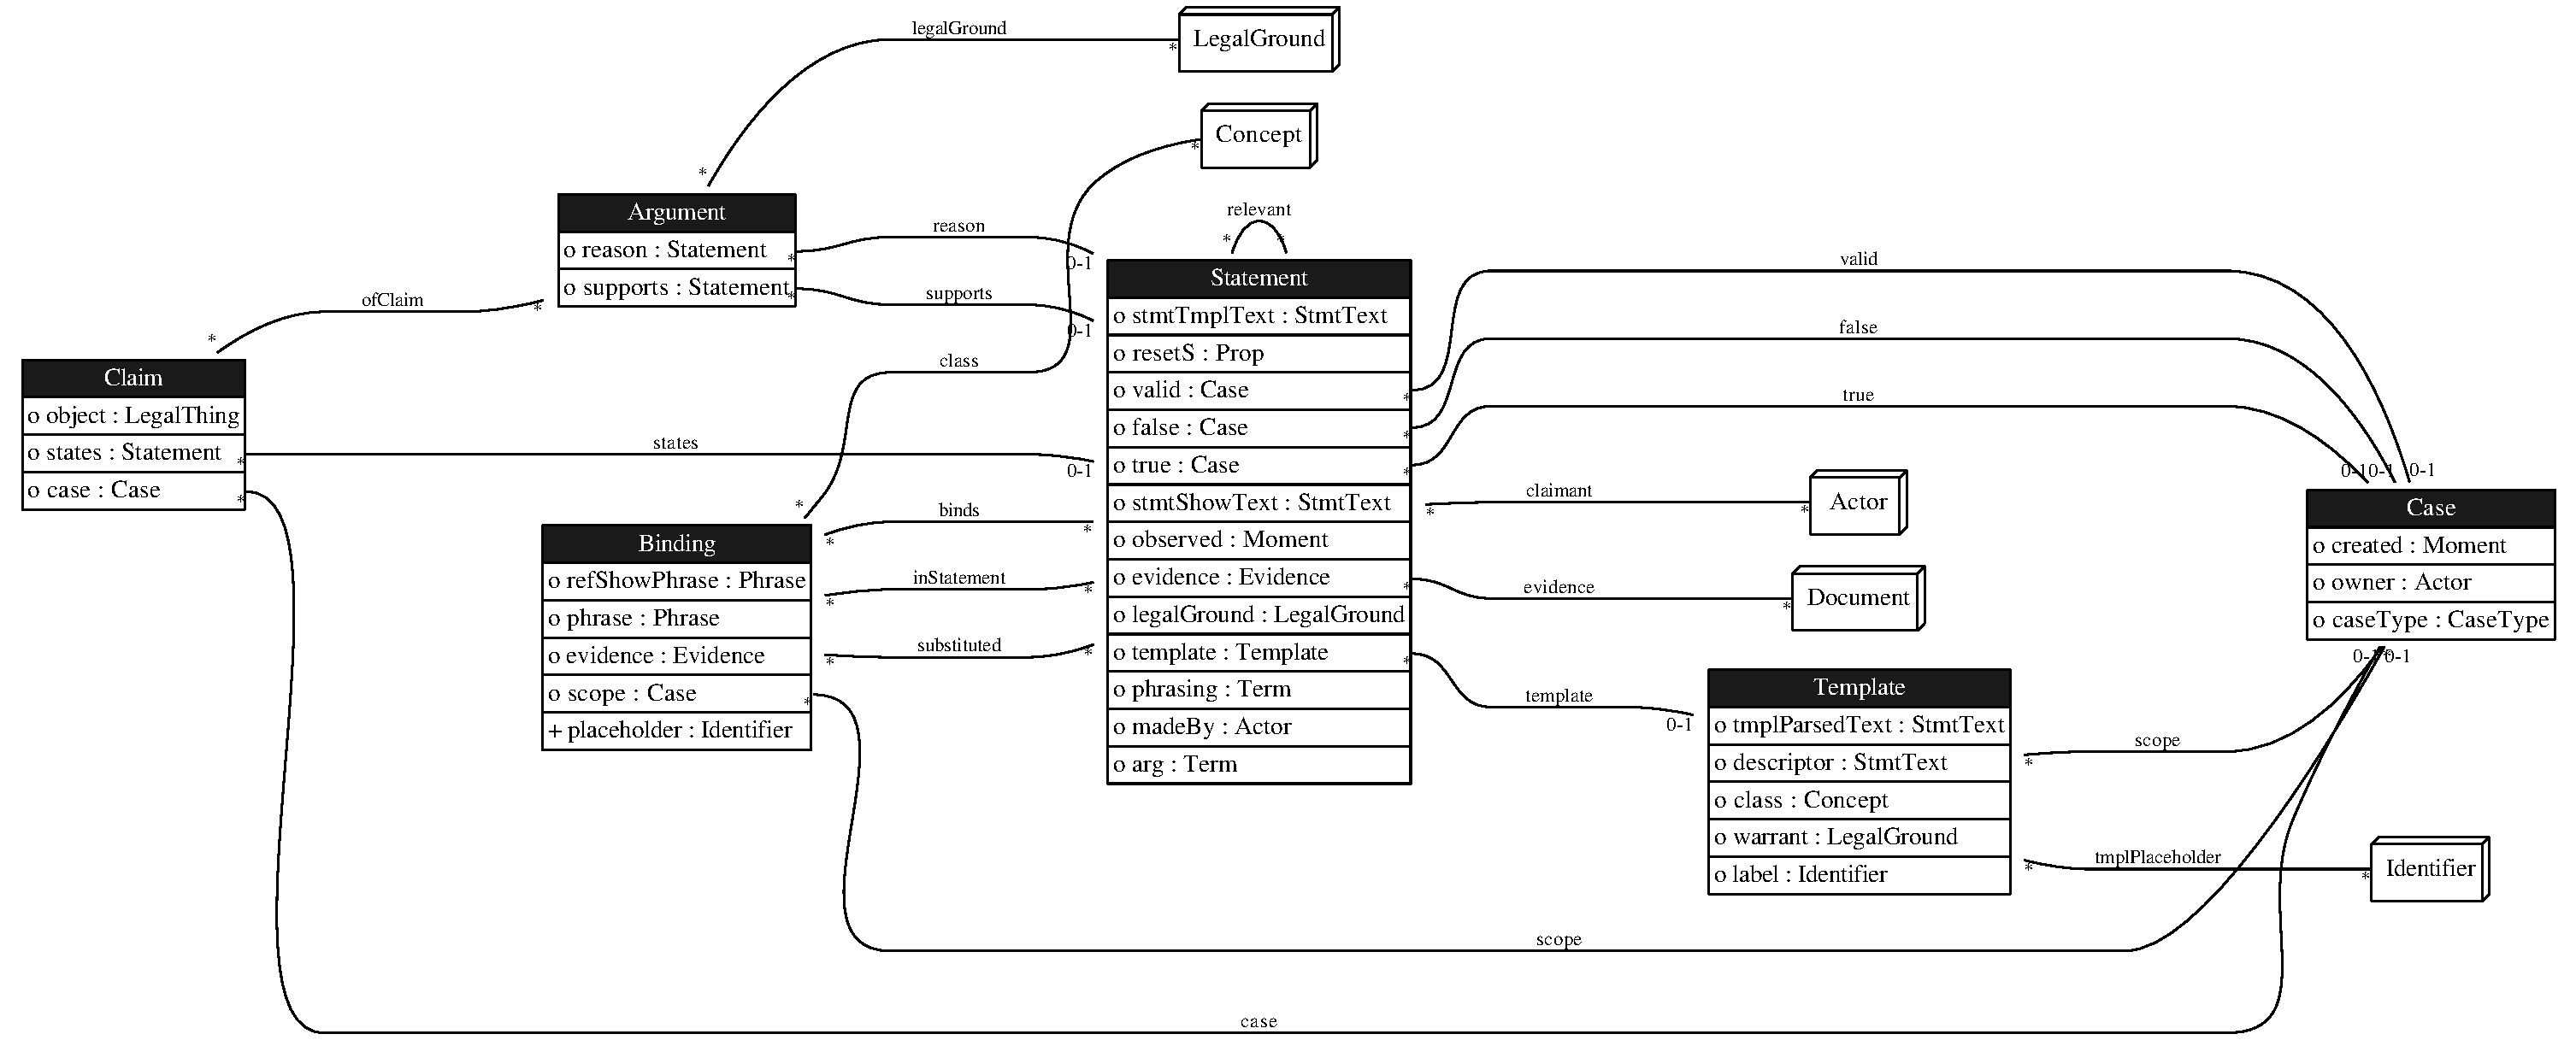
\includegraphics[angle=90,scale=.357]{LogicalDataModel.pdf}
% \end{center}
% \caption{Conceptual data model (from section~\ref{sct:Conceptual analysis})}
% \label{fig:conceptual model}
% \end{figure}

\section{Bibliography}
\bibliographystyle{elsarticle-harv}
\bibliography{doc}


\end{document}
